\documentclass{article}
\usepackage{nips15submit_e,times}
\usepackage{hyperref}
\usepackage{url}
\usepackage{graphicx}
\usepackage{latexsym}

\title{Weekly Report(March.19,2019-April.17,2019)}

\newcommand{\fix}{\marginpar{FIX}}
\newcommand{\new}{\marginpar{NEW}}


\begin{document}

\maketitle
\begin{abstract}
	During these weeks, I finished assignment3. I learned RNN, LSTM and some other interesting models. And I also modified the last part of Pytorch.ipnb in assignment2.
\end{abstract}

\section{Learned}
After finishing all the thing about them, I have to say, it's easy to finish code if you know the formula. But it'e hard to understand how they work and why they can make it. 
\subsection{RNN}
\subsubsection{Introduction}
Recurrent Neural Network. It's a typical model to address squential data, such as videos, sentences, music and so on.\\
\begin{figure}[h]
	\centering  %插入的图片居中表示
	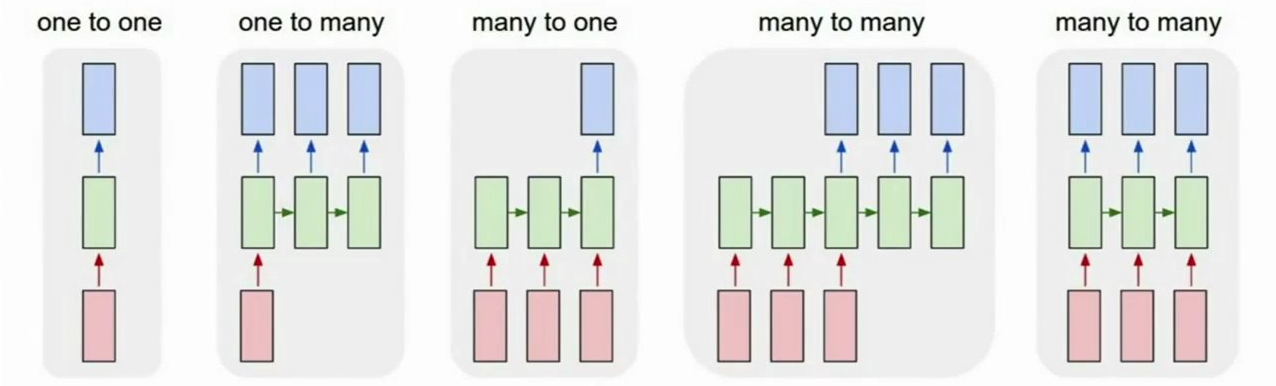
\includegraphics[width=1\textwidth]{1.png} 
	\caption{Different kinds of RNN}  %图片的名称
	\label{fig:f1}   %标签,用作引用
\end{figure}

Formula:

for each hidden layer:
\begin{center}
${\displaystyle h_t=f_w(h_{t-1}, x_t)=tanh(Wh_{t-1}*h_{t-1}+Wx*X+b)}$\\
${y_t=W_{hy}h_t}$
\end{center}
${h_t}$is the new state, while ${h_{t-1}}$is the old state, and ${x_t}$ is input of this timestep. ${f_w}$ is some function with parameters W, the right part of the equation is the function used in homework. ${y_t}$ will be used when calculating loss.

\begin{figure}[htbp]
	\centering  %插入的图片居中表示
	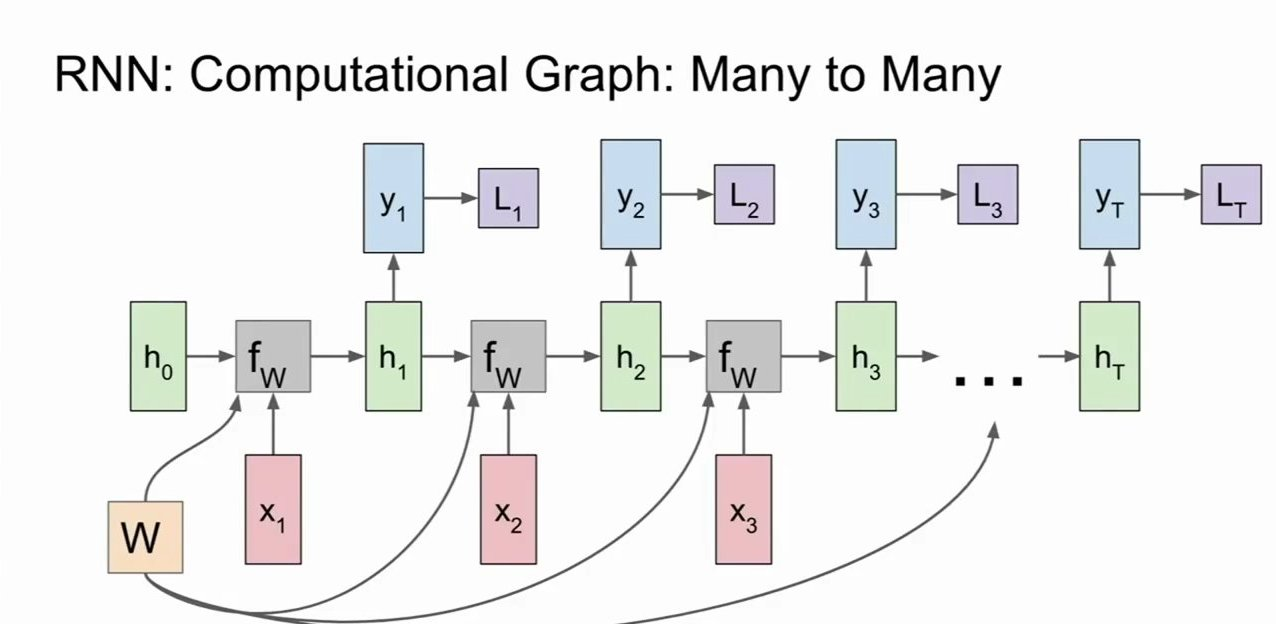
\includegraphics[width=0.8\textwidth]{2.jpg} 
	\caption{Typical many-to-many model}  %图片的名称
	\label{fig:f2}   %标签,用作引用
\end{figure}

\subsubsection{My work}
Actually It's much more easier than other parts, so I will just show the result.

\begin{figure}[htbp]
	\centering  %插入的图片居中表示
	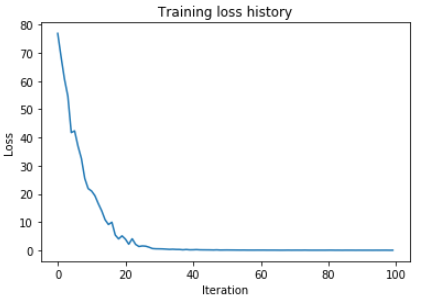
\includegraphics[width=0.8\textwidth]{3.png} 
	\caption{loss}  %图片的名称
	\label{fig:f3}   %标签,用作引用
\end{figure}

\begin{figure}[htbp]
	\centering
	\begin{minipage}[t]{0.5\textwidth}
		\centering
		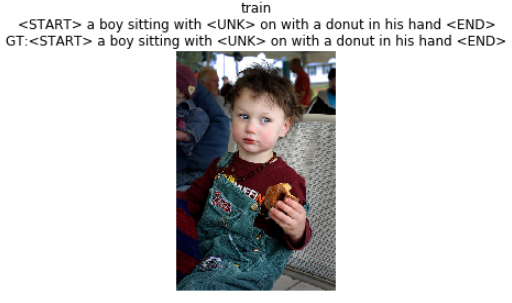
\includegraphics[width=1.0\textwidth]{4.png}
	%	\caption{ab}
	\end{minipage}
	\begin{minipage}[t]{0.45\textwidth}
		\centering
		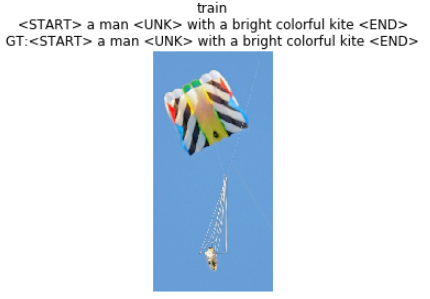
\includegraphics[width=1.0\textwidth]{5.png}
	\end{minipage}
	\caption{trained result}
\end{figure}

\subsection{LSTM}
\subsubsection{Introduction}
Long Short Term Memory, is slightly fancier recurrence relationfor RNN. It's designed to solve the problem of vanishing and exploding gradients.

Formula:

\begin{center}
	$\left( \begin{array}{ccc} i\\f\\o\\g\end{array} \right)
	=\left( \begin{array}{ccc} \sigma\\\sigma\\\sigma\\tanh\end{array} \right)
	W\left( \begin{array}{ccc} h_{t-1}\\x_t \end{array} \right)$

	${\displaystyle c_t=f\odot c_{t-1}+i\odot g}$
	
	${\displaystyle h_t=o \odot tanh(c_t)}$
\end{center}

In this formulas, \textsl{i} means \textsl{input\_gate}, \textsl{f} means \textsl{forget\_gate}, \textsl{o} means \textsl{output\_gate}, while \textsl{g} doesn't have a good name.

\subsubsection{My work}
The implementation is the same as RNN, so I will still say nothing about it.


\begin{figure}[htbp]
	\centering  %插入的图片居中表示
	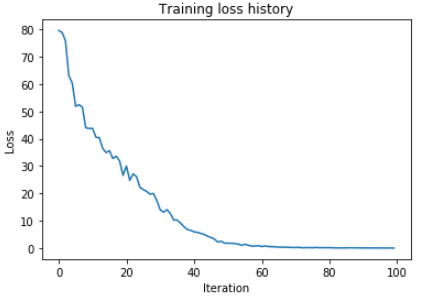
\includegraphics[width=.7\textwidth]{6.png} 
	\caption{Final result}  %图片的名称
	\label{fig:f6}   %标签,用作引用
\end{figure}

\begin{figure}[htbp]
	\centering
	\begin{minipage}[t]{0.5\textwidth}
		\centering
		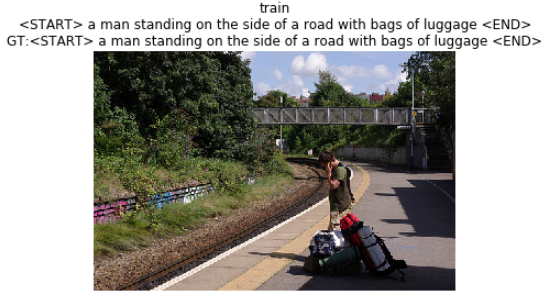
\includegraphics[width=1.0\textwidth]{7.png}
	\end{minipage}
	\begin{minipage}[t]{0.4\textwidth}
		\centering
		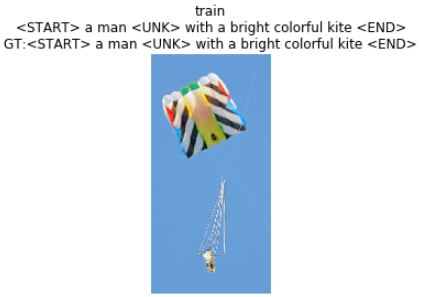
\includegraphics[width=1.0\textwidth]{8.png}
	\end{minipage}
	\caption{trained results} 
\end{figure}

\section{Modification}
After finishing assignment3, I think back "open-ended challenge" in assignment2. Since it really attracted me and I think I can find a better model to get better grade.

I try to modify the model for several trials, I finally get about 80\% accuracy. But I have some questions showed below.

\begin{figure}[htbp]
	\centering  %插入的图片居中表示
	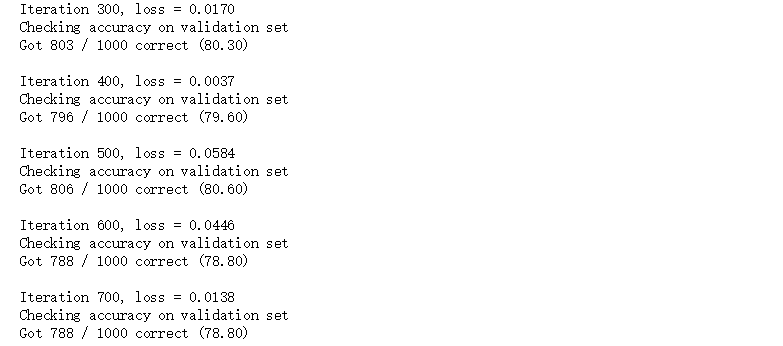
\includegraphics[width=0.8\textwidth]{9.png} 
	\caption{open-ended challenge accuracy}  %图片的名称
	\label{fig:f9}   %标签,用作引用
\end{figure}

\section{Understanding}
RNN addresses sequential words in the homework. In order to predict next layer's state, it will use all of the previous state as input. It works very well. However, it has the problem of vanishing and exploding gradients. That's why LSTM exists. LSTM will forget part of previous hidden state, which makes the network work better. 

\textbf{Question}: As training goes on, I come to confuse about the relation between an actual layer and its functions. For example, why adding convolutional layers in a CNN will get better performance? I know there must be some scientific basis, so how to use this basis if I want to improve a model?

\section{Plan}
I need to focus on my professional courses.
\end{document}